% Template:     Informe LaTeX
% Documento:    Archivo principal
% Versión:      8.4.4 (02/12/2025)
% Codificación: UTF-8
%
% Autor: Pablo Pizarro R.
%        pablo@ppizarror.com
%
% Manual template: [https://latex.ppizarror.com/informe]
% Licencia MIT:    [https://opensource.org/licenses/MIT]

% CREACIÓN DEL DOCUMENTO
\documentclass[
	spanish, % Idioma: spanish, english, etc.
	letterpaper, oneside
]{article}

% INFORMACIÓN DEL DOCUMENTO
\def\documenttitle {Actividad 2}
\def\documentsubtitle {Construyamos un resolver}
\def\documentsubject {DNS}

\def\documentauthor {María Moya G., M. Fernando Saavedra}
\def\coursename {Redes}
\def\coursecode {CC4303}

\def\universityname {Universidad de Chile}
\def\universityfaculty {Facultad de Ciencias Físicas y Matemáticas}
\def\universitydepartment {Departamento de Ciencias de la Computación}
\def\universitydepartmentimage {departamentos/dcc}
\def\universitydepartmentimagecfg {height=1.57cm}
\def\universitylocation {Santiago de Chile}

% INTEGRANTES, PROFESORES Y FECHAS
\def\authortable {
	\begin{tabular}{ll}
		Integrantes:
		& \begin{tabular}[t]{l}
			María Moya G. \\
			M. Fernando Saavedra
		\end{tabular} \\
		Profesor:
		& \begin{tabular}[t]{l}
			Ivana Bachmann
		\end{tabular} \\
		Auxiliar:
		& \begin{tabular}[t]{l}
			Julián Ferreira
		\end{tabular} \\
		Ayudantes:
		& \begin{tabular}[t]{l}
			Diego García G. \\
			Valeria Serrano
		\end{tabular} \\
		& \\
		\multicolumn{2}{l}{Fecha de realización: \today} \\
		% TODO: confirmar la fecha de entrega de la actividad 2
		\multicolumn{2}{l}{Fecha de entrega: \today} \\
		\multicolumn{2}{l}{\universitylocation}
	\end{tabular}
}

% IMPORTACIÓN DEL TEMPLATE
\input{template}

% CONVENCIÓN TIPOGRÁFICA
% El cuerpo del informe se compone en una sola fuente: no se usa monoespaciado,
% negrita ni cursiva para destacar nombres de archivo, funciones, comandos, IPs
% ni vocabulario del protocolo. La tipografía solo cambia dentro de los bloques
% verbatim, que reproducen salidas literales de dig y del modo debug. Las cuatro
% macros se conservan como marcas semánticas y no producen ningún cambio visual.
\newcommand{\code}[1]{#1}              % identificadores, funciones, archivos, comandos, IPs
\newcommand{\rr}[1]{#1}               % tipos de registro DNS (A, NS, CNAME, SOA)
\newcommand{\msgsec}[1]{#1}           % secciones del mensaje DNS (Question, Answer, Authority, Additional)
\newcommand{\field}[1]{#1}            % campos y flags del encabezado (ID, QR, RD, QDCOUNT, ANCOUNT)

% INICIO DE PÁGINAS
\begin{document}

% PORTADA
\templatePortrait

% CONFIGURACIÓN DE PÁGINA Y ENCABEZADOS
\templatePagecfg

% RESUMEN O ABSTRACT
%\begin{abstractd}
%	\lipsum[1] % Párrafo ejemplo, se puede borrar
%\end{abstractd}

% TABLA DE CONTENIDOS - ÍNDICE
\templateIndex

% CONFIGURACIONES FINALES
\templateFinalcfg

% ======================= INICIO DEL DOCUMENTO =======================

\section{Consultas preliminares}
Se pide comparar la IP que entrega dig al preguntarle a 1.1.1.1 por example.com con lo que se obtiene en la sección anterior usando dnslib. Ambas consultas devuelven el mismo par de direcciones:

\begin{verbatim}
% dig @1.1.1.1 example.com
;; flags: qr rd ra ad; QUERY: 1, ANSWER: 2, AUTHORITY: 0, ADDITIONAL: 1
;; OPT PSEUDOSECTION:
; EDNS: version: 0, flags:; udp: 1232
;; ANSWER SECTION:
example.com.            215     IN      A       104.20.23.154
example.com.            215     IN      A       172.66.147.243

% python3 dns_socket.py
;; flags: qr rd ra; QUERY: 1, ANSWER: 2, AUTHORITY: 0, ADDITIONAL: 0
;; ANSWER SECTION:
example.com.            167     IN      A       104.20.23.154
example.com.            167     IN      A       172.66.147.243
\end{verbatim}

Las respuestas se diferencian en tres detalles: el TTL, 215 contra 167 segundos; el flag ad, presente solo en la de dig; y la sección Additional, que en la de dig trae un registro OPT de EDNS y en la del script viene vacía.

\section{Diseño del resolver}

\subsection{Socket y recepción de mensajes}
El socket debe ser No orientado a conexión, luego se utiliza AF\_INET y SOCK\_DGRAM, es decir, UDP sobre IPv4. Esto es porque una consulta DNS prioriza una mínima latencia, y las respuestas son simples, por lo que no requiere la complejidad y demora adicionales de TCP. Además, un solo socket UDP atiende a todos los clientes: recvfrom entrega junto al mensaje la dirección de quien lo envió, que es a donde después se responde con sendto.

El socket se enlaza a (0.0.0.0, 8000), lo que equivale a (IP\_VM, 8000) visto desde el host y además permite consultar por loopback durante el desarrollo. La recepción es un loop con recvfrom y un buffer de 4096 bytes. Cada mensaje recibido se imprime tal como llega, sin decode(), porque un mensaje DNS es binario y no texto.

Un detalle a considerar es el tamaño, sin EDNS un mensaje no puede pasar de 512 bytes, y cuando la respuesta no cabe el servidor enciende el flag TC para que el cliente reintente sobre TCP. El resolver no implementa ese reintento, y en el experimento 3 se ve el efecto concreto.

\subsection{Parseo de mensajes DNS}
La función de parseo recibe los bytes crudos y devuelve un diccionario con Qname, ANCOUNT, NSCOUNT, ARCOUNT y las tres secciones del mensaje, Answer, Authority y Additional, que es exactamente la estructura sugerida en el enunciado. El trabajo pesado lo hace DNSRecord.parse de dnslib; la función se limita a extraer esos campos y a devolver un diccionario con una clave de error si el mensaje no se puede parsear.

Se eligió un diccionario porque el programa principal solo necesita acceso por nombre a unos pocos campos: Qname para consultar el caché, y el resto para imprimir la estructura en pantalla. Las secciones se guardan como listas de texto, suficiente para mostrarlas. La lógica de resolución, en cambio, no usa este diccionario sino el objeto DNSRecord directamente, porque necesita distinguir tipos de registro y leer direcciones, y ahí conviene conservar los objetos de dnslib en vez de su representación en texto.

\subsection{Resolución iterativa: resolver()}
La firma es resolver(mensaje\_consulta: bytes, ip\_addr=ROOT\_IP, ns\_name="."), donde el tercer parámetro solo transporta el nombre del Name Server para el modo debug y tiene valor por defecto, de modo que la función se puede invocar con la firma que pide el enunciado. La constante ROOT\_IP es 198.41.0.4.

\begin{figure}[ht]
	\centering
	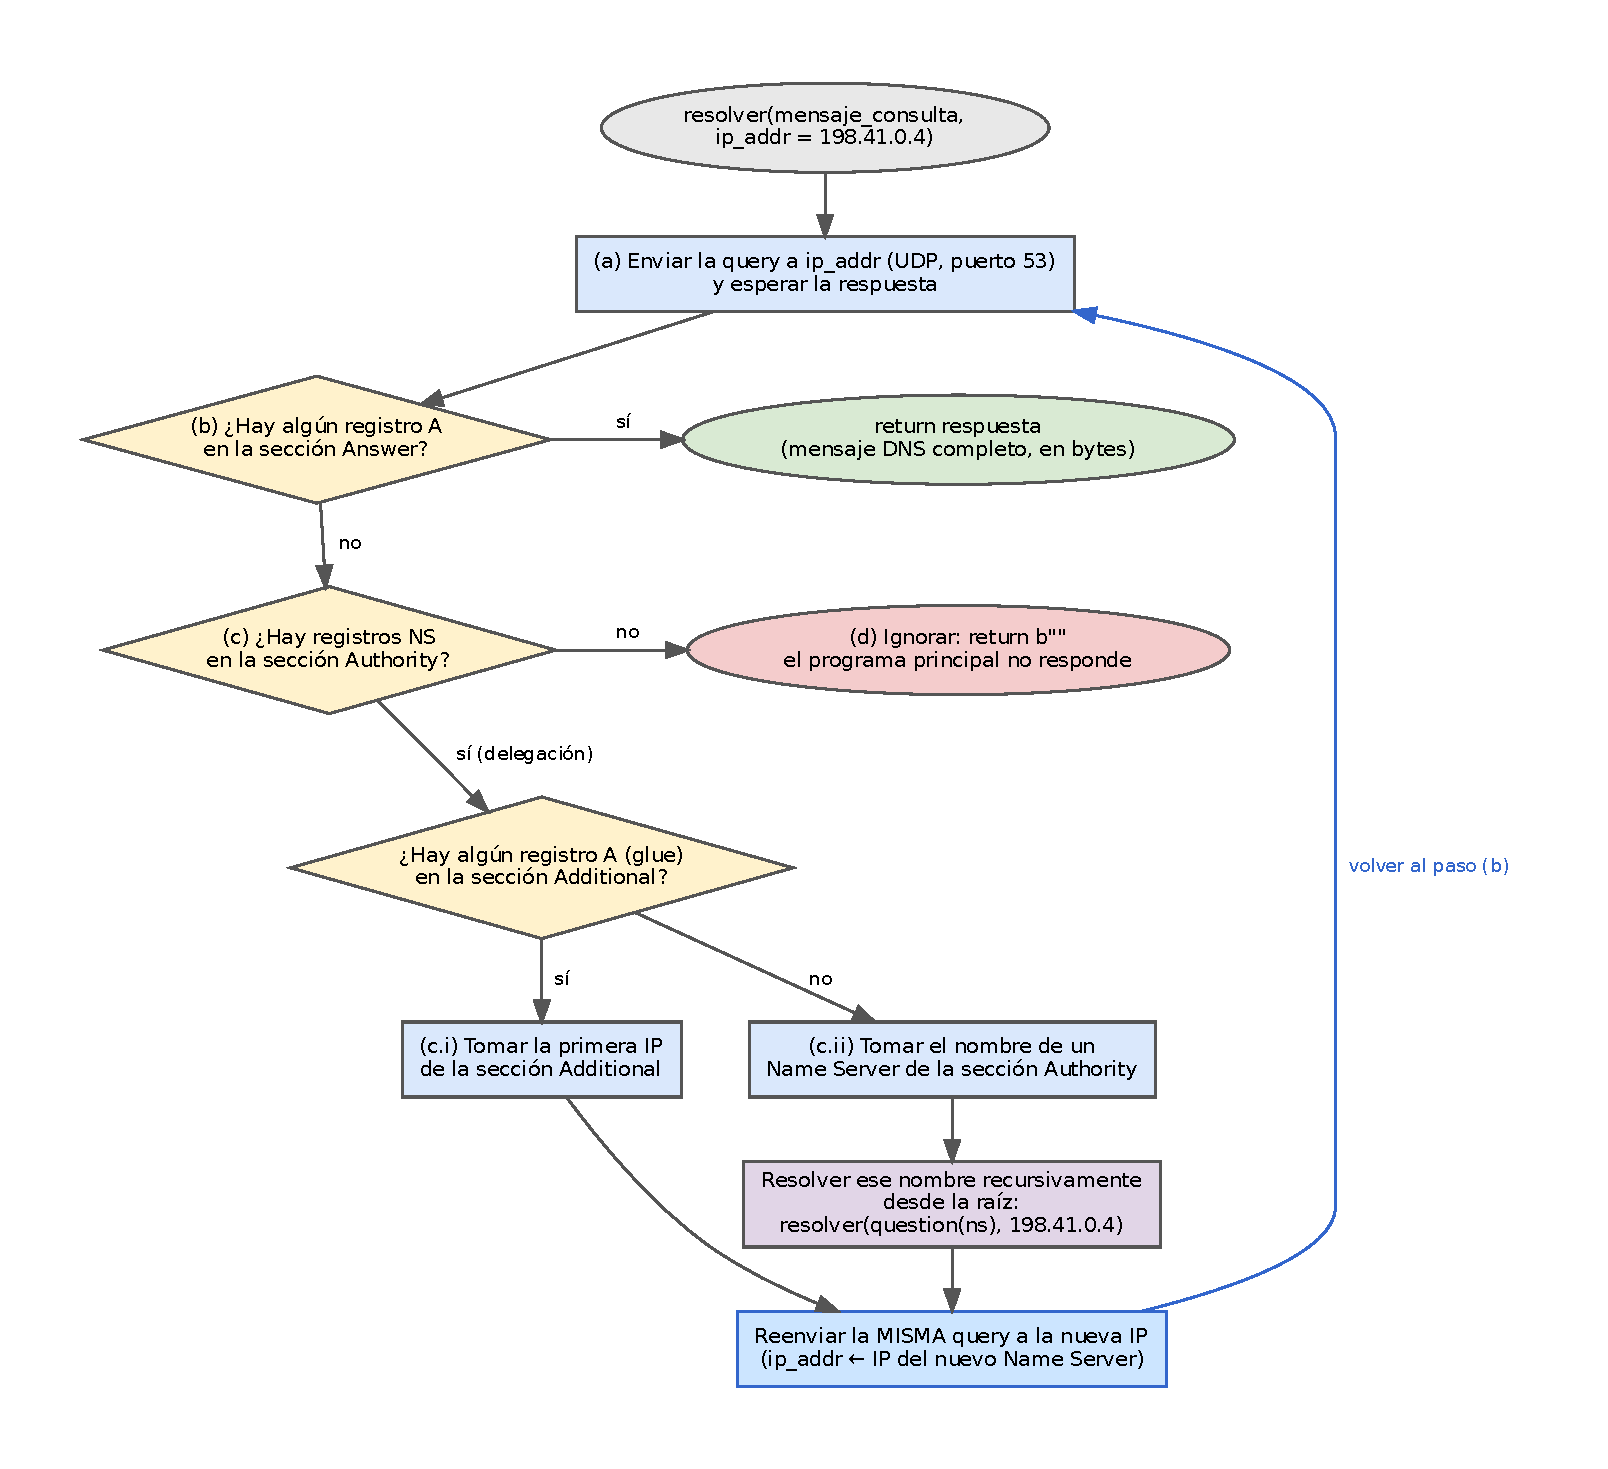
\includegraphics[width=0.82\textwidth]{img/algoritmo_resolver.pdf}
	\caption{Procedimiento del punto 3 del enunciado, tal como está implementado.}
	\label{fig:algoritmo}
\end{figure}

Dos detalles del recorrido merecen atención. El primero es que lo que viaja por la cadena de delegación es siempre la consulta original del cliente, sin modificar: solo cambia la IP a la que se envía. Eso es lo que permite devolverle a dig el mensaje del servidor autoritativo tal como llegó, con su mismo identificador y su misma sección Question. El segundo es que la recursión del caso (c.ii) no es sobre el dominio consultado sino sobre el nombre del Name Server, y parte de nuevo desde la raíz; la prueba de cc4303.bachmann.cl muestra esa rama en funcionamiento.

El caso (d), ignorar cualquier otra forma de respuesta, es la fuente de las dos limitaciones que documentan los experimentos 1 y 2: una respuesta con un CNAME y sin registros A se confunde con una delegación y provoca un ciclo, y una respuesta negativa se descarta en vez de reenviarse al cliente.

\subsection{Modo debug}
Se controla con la constante DEBUG al inicio del archivo. Por cada consulta interna se imprime una línea con los tres datos que pide el enunciado, el dominio consultado, el nombre del Name Server y su dirección IP:

\begin{verbatim}
(debug) Consultando 'www.uchile.cl' a '.' con dirección IP '198.41.0.4'
\end{verbatim}

A eso se agregan dos mensajes propios: uno que avisa cuando la sección Additional no trae glue y hay que resolver primero el nombre del Name Server, y otro que indica si la consulta se resolvió desde el caché o no. Las trazas de las secciones anteriores son la salida real de este modo.

\subsection{Caché}
La regla del enunciado no es la de un caché DNS ordinario: se guardan los 3 dominios más repetidos dentro de las últimas 20 consultas recibidas. Eso son dos estructuras. Una lista conserva las últimas 20 consultas, descartando la más antigua cuando se pasa de ese largo, y un Counter sobre esa lista entrega los tres dominios más frecuentes. Un diccionario aparte asocia cada uno de esos dominios con su dirección IP.

Toda consulta que llega se busca primero en ese diccionario. Después de responder, venga la respuesta de la red o del propio caché, se agrega el dominio al historial, se recalculan los tres más frecuentes, se guarda la IP del dominio actual si quedó entre ellos y se borran las entradas que salieron. Esa última parte es la que hace que el caché expulse, y no solo acumule.

Se guarda la dirección IP y no el mensaje completo, que es lo que el enunciado pide, y no se guarda el TTL, porque la regla de permanencia la fija la ventana de 20 consultas y no el tiempo. Las consecuencias visibles de ambas decisiones aparecen en la sección Uso del caché.

\section{Pruebas de funcionalidad}
Las pruebas se ejecutaron con el resolver corriendo en la máquina virtual, con su socket UDP enlazado a (0.0.0.0, 8000) y consultado desde el anfitrión: IP\_VM fue 192.168.2.5 y el anfitrión 192.168.2.4. La VM corre Python 3.11.2 con dnslib 0.9.23 y el cliente es dig 9.20.27. El resolver se reinició antes de cada prueba, de modo que todas parten con el caché vacío. Las salidas completas están en el directorio pruebas/ del repositorio, un archivo por prueba; aquí van solo los fragmentos pertinentes. La versión del paso 1, que solo recibe e imprime el mensaje sin decodificar, deja a dig en connection timed out tal como anticipa el enunciado.

\subsection{eol.uchile.cl}
La consulta devuelve 12 respuestas en la sección Answer: un registro CNAME que apunta eol.uchile.cl a oeol-c.uchile.cl, y once registros A de la forma 146.83.63.X asociados a ese nombre canónico.

\begin{verbatim}
% dig -p8000 @192.168.2.5 eol.uchile.cl
;; flags: qr aa rd; QUERY: 1, ANSWER: 12, AUTHORITY: 0, ADDITIONAL: 1
;; ANSWER SECTION:
eol.uchile.cl.          3600    IN      CNAME   oeol-c.uchile.cl.
oeol-c.uchile.cl.       3600    IN      A       146.83.63.77
oeol-c.uchile.cl.       3600    IN      A       146.83.63.40
    [... nueve registros A más, todos 146.83.63.X ...]
;; Query time: 185 msec
\end{verbatim}

La cadena recorrida fue la raíz, cl2-tld.d-zone.ca (185.159.198.56) y ns1.uchile.cl (200.89.70.3). El nombre consultado no tiene un registro A propio, pero el servidor autoritativo de uchile.cl resuelve el CNAME dentro de su misma zona y entrega ambas cosas en un solo mensaje; como el resolver retorna ese mensaje sin modificar, las doce respuestas llegan íntegras a dig.

\subsection{Uso del caché}
La segunda consulta a eol.uchile.cl entrega la misma dirección, 146.83.63.77, pero esta vez la responde el caché: dig reporta Query time: 0 msec y el modo debug lo anuncia.

\begin{verbatim}
% dig -p8000 @192.168.2.5 eol.uchile.cl
;; Warning: query response not set
;; flags: rd ad; QUERY: 1, ANSWER: 1, AUTHORITY: 0, ADDITIONAL: 1
eol.uchile.cl.          0       IN      A       146.83.63.77
;; Query time: 0 msec
\end{verbatim}

{\scriptsize
\begin{verbatim}
(debug) [CACHE HIT] Respuesta entregada desde caché para 'eol.uchile.cl', de IP '146.83.63.77'
\end{verbatim}
}

La respuesta desde caché no es idéntica a la original porque lo que se guarda no es el mensaje completo, sino la primera dirección de tipo A, que al llegar la repetición se monta como único registro de Answer sobre el mensaje de consulta del cliente. De ahí las diferencias: llega un solo registro A en vez de doce, se pierde el CNAME intermedio, el TTL queda en 0 porque es el valor por defecto de RR en dnslib, y el bit QR del encabezado sigue valiendo 0, que es lo que dig señala como query response not set. Marcar ese bit en 1 antes de serializar la respuesta la deja con la misma forma que la que viene de la red. Las respuestas que no pasan por el caché no tienen este problema: son el mensaje del servidor autoritativo reenviado sin modificar.

\subsection{www.uchile.cl}
El resolver entrega 200.89.76.36, la misma dirección que responde Cloudflare.

\begin{verbatim}
% dig @1.1.1.1 www.uchile.cl
;; flags: qr rd ra; QUERY: 1, ANSWER: 1, AUTHORITY: 0, ADDITIONAL: 1
www.uchile.cl.          300     IN      A       200.89.76.36
;; Query time: 8 msec

% dig -p8000 @192.168.2.5 www.uchile.cl
;; flags: qr aa rd; QUERY: 1, ANSWER: 1, AUTHORITY: 0, ADDITIONAL: 1
www.uchile.cl.          300     IN      A       200.89.76.36
;; Query time: 162 msec
\end{verbatim}

Las dos difieren en dos detalles que delatan su origen. La de Cloudflare trae el flag ra, recursion available, y tarda 8 ms, porque es un resolver recursivo que ya tenía el nombre en su caché; la nuestra trae aa, authoritative answer, y tarda 162 ms, porque es el mensaje que acaba de emitir ns1.uchile.cl tras recorrer la cadena completa desde la raíz.

\subsection{cc4303.bachmann.cl}
El resolver entrega 104.248.65.245. Esta prueba ejercita la rama recursiva del paso 3.c.ii: el TLD cl delega en ns1.digitalocean.com, un nombre fuera de la zona .cl, de modo que la respuesta no puede traer glue en Additional y hay que resolver primero la IP de ese Name Server.

{\scriptsize
\begin{verbatim}
(debug) [CACHE MISS] 'cc4303.bachmann.cl' no está en caché. Resolviendo...
(debug) Consultando 'cc4303.bachmann.cl' a '.' con dirección IP '198.41.0.4'
(debug) Consultando 'cc4303.bachmann.cl' a 'cl2-tld.d-zone.ca' con dirección IP '185.159.198.56'
(debug) Sin glue en Additional; resolviendo primero la IP de 'ns1.digitalocean.com'
(debug) Consultando 'ns1.digitalocean.com' a '.' con dirección IP '198.41.0.4'
(debug) Consultando 'ns1.digitalocean.com' a 'l.gtld-servers.net' con dirección IP '192.41.162.30'
(debug) Consultando 'ns1.digitalocean.com' a 'kim.ns.cloudflare.com' con dirección IP '108.162.192.126'
(debug) Consultando 'cc4303.bachmann.cl' a 'ns1.digitalocean.com' con dirección IP '172.64.52.210'
\end{verbatim}
}

Las cuatro líneas del medio son la resolución anidada: el resolver se llama a sí mismo con ns1.digitalocean.com, parte de nuevo desde la raíz, baja por el TLD com y obtiene 172.64.52.210. Recién entonces reenvía la consulta original, sin modificar, a esa dirección. Los 813 ms que tomó la consulta, contra los 162 ms de www.uchile.cl, son el costo de esa segunda cadena completa.

\subsection{Política del caché}
Dos pruebas adicionales verifican la regla que define el caché: los 3 dominios más repetidos dentro de las últimas 20 consultas. Con el caché recién iniciado se consultaron cuatro dominios distintos y luego se repitió la secuencia.

{\scriptsize
\begin{verbatim}
vuelta 1   MISS www.uchile.cl   MISS cc4303.bachmann.cl   MISS example.com   MISS eol.uchile.cl
vuelta 2   HIT  www.uchile.cl   HIT  cc4303.bachmann.cl   HIT  example.com   MISS eol.uchile.cl
vuelta 3   MISS eol.uchile.cl   HIT  eol.uchile.cl        HIT  eol.uchile.cl
vuelta 4   MISS example.com
\end{verbatim}
}

Los tres primeros dominios quedan en caché y el cuarto no, porque con todas las frecuencias empatadas en 1 el desempate lo gana el que entró antes. En la vuelta 3, eol.uchile.cl pasa a ser el más frecuente y entra al caché desplazando a example.com, que en la vuelta 4 vuelve a ser MISS: el caché no solo agrega, también expulsa.

La segunda prueba verifica el largo de la ventana. Tras veinte consultas a www.uchile.cl (la primera resolviendo, las diecinueve siguientes desde el caché) y otras veinte a cc4303.bachmann.cl, la consulta número 41, de nuevo por el primer dominio, es MISS: las repeticiones del segundo lo empujaron fuera de la ventana y su frecuencia bajó a 0.

\section{Experimentos}

\subsection{www.webofscience.com}
El resolver no resuelve este dominio, y tampoco falla: se queda dando vueltas. dig corta por timeout sin recibir nada, mientras el modo debug repite indefinidamente el mismo ciclo de cinco líneas.

La causa está en lo que devuelve el último servidor de la cadena. Consultado directamente, ns-1010.awsdns-62.net responde con dos CNAME en Answer, el conjunto NS de la zona en Authority y Additional vacía:

{\scriptsize
\begin{verbatim}
ANCOUNT=2  NSCOUNT=4  ARCOUNT=0
-- Answer --
   www.webofscience.com.      CNAME  www-us.webofscience.com.
   www-us.webofscience.com.   CNAME  www-us.webofscience.com.cdn.cloudflare.net.
-- Authority --
   webofscience.com.          NS     ns-1010.awsdns-62.net.
   webofscience.com.          NS     ns-1384.awsdns-45.org.
   webofscience.com.          NS     ns-1673.awsdns-17.co.uk.
   webofscience.com.          NS     ns-342.awsdns-42.com.
-- Additional --   (vacía)
\end{verbatim}
}

Esa respuesta es final, no una delegación, pero tiene exactamente la forma que el resolver interpreta como delegación. El procedimiento del paso 3 pregunta primero si hay algún registro A en Answer, y no lo hay, hay dos CNAME; después pregunta si hay registros NS en Authority, y sí los hay, porque Route 53 adjunta el conjunto NS de la zona también cuando la respuesta es final. Como Additional viene vacía, el resolver toma el primer nombre de Authority, lo resuelve desde la raíz, obtiene su IP y le reenvía la consulta original al mismo servidor que acaba de responder. La respuesta es idéntica y el ciclo se repite.

Cada vuelta agrega un marco a la pila de Python, así que con el límite de recursión por defecto el proceso termina cayendo con RecursionError; se verificó bajando el límite a 40 para observar el desenlace en segundos en vez de en minutos. Como el resolver es de un solo hilo, mientras dura el ciclo no atiende a nadie más, y cuando cae deja de atender del todo. Esa es la limitación concreta de ignorar los tipos de respuesta no contemplados en el paso 3.d: el problema no es solo no saber resolver un CNAME, sino que una respuesta perfectamente válida se confunde con una delegación.

El arreglo tiene dos partes, y conviene hacer las dos. La primera es seguir el CNAME: si Answer trae un CNAME para el nombre consultado y ningún registro A, reiniciar la resolución con el nombre canónico y entregar al cliente la cadena completa, los CNAME recorridos más los registros A finales, con el QNAME original en la sección Question. Es lo que hace 1.1.1.1, que para este mismo dominio devuelve los dos CNAME y las dos direcciones de Cloudflare en un solo mensaje. La segunda es cortar la delegación que no avanza: si la IP a la que se va a preguntar es la misma a la que ya se preguntó, o si se supera una profundidad máxima, devolver un mensaje vacío. Así el dominio seguiría sin resolverse, pero el resolver fallaría rápido y seguiría atendiendo al resto.

\subsection{www.cc4303.bachmann.cl}
Con nuestro resolver la consulta no obtiene respuesta: dig corta por timeout y en la VM queda el mensaje ``No se pudo obtener una respuesta del resolver''. Con 1.1.1.1, en cambio, la consulta sí obtiene respuesta, y es una respuesta negativa:

\begin{verbatim}
% dig @1.1.1.1 www.cc4303.bachmann.cl
;; ->>HEADER<<- opcode: QUERY, status: NXDOMAIN, id: 4873
;; flags: qr rd ra; QUERY: 1, ANSWER: 0, AUTHORITY: 1, ADDITIONAL: 1
;; AUTHORITY SECTION:
bachmann.cl.  1800  IN  SOA  ns1.digitalocean.com. hostmaster.bachmann.cl.
                             0 10800 3600 604800 1800
\end{verbatim}

Lo que habríamos esperado es justamente eso, un NXDOMAIN: el nombre www.cc4303.bachmann.cl no existe, porque en la zona bachmann.cl el nombre cc4303 es un host y no una subzona con un www adentro.

Nuestro resolver sí llega al servidor que conoce la respuesta. El modo debug muestra la cadena completa, incluida la resolución anidada de ns1.digitalocean.com, y termina preguntándole a la IP correcta; es la respuesta la que se descarta. ns1.digitalocean.com contesta con RCODE 3, ANCOUNT 0 y un registro SOA en Authority, cuyo último campo, el minimum, es el TTL con el que se puede cachear la negación (RFC 2308). El resolver del paso 3 solo sabe reconocer dos formas de respuesta, un registro A en Answer o registros NS en Authority, y una respuesta negativa no es ninguna de las dos: cae en el caso 3.d, la función retorna vacío, el programa principal decide no enviar nada y dig se queda esperando. Visto desde el protocolo, la diferencia entre ambos comportamientos es la que hay entre decir ``no existe'' y no decir nada. Devolver al cliente, tal como llegó, toda respuesta con RCODE distinto de 0 basta para cerrar la brecha.

\subsection{Estabilidad de los Name Servers consultados}
Se resolvió www.uchile.cl cinco veces, reiniciando el resolver antes de cada consulta para que el caché no interfiriera. La cadena fue idéntica las cinco veces: la raíz 198.41.0.4, después cl2-tld.d-zone.ca en 185.159.198.56 y por último ns1.uchile.cl en 200.89.70.3.

Sí son siempre los mismos Name Servers, por tres razones encadenadas. La IP de la raíz está fija en el código, así que el primer salto no puede variar; un resolver real conoce las trece raíces y elige entre ellas. En cada delegación el resolver toma el primer registro A de la sección Additional, sin sortear ni medir latencias, de modo que la elección es una función determinista de la respuesta que llegó. Y los servidores padres entregan esa sección en un orden estable ante la misma consulta: repitiendo diez veces la consulta directamente contra la raíz, el primer registro A fue siempre el mismo, tanto para www.uchile.cl como para example.com.

Ese orden, sin embargo, no es universal ni alfabético: cambia según el nombre consultado. Para los dominios .com la raíz ofrece 13 servidores NS pero solo alcanza a incluir 6 registros A en Additional, y cuál queda primero depende del nombre, l.gtld-servers.net para example.com y ns1.digitalocean.com, m.gtld-servers.net para ns-1010.awsdns-62.net. La razón del recorte es el tamaño: la respuesta para example.com ocupa 489 de los 512 bytes que admite un mensaje DNS sin EDNS y llega con el flag TC encendido, avisando que quedaron registros fuera; la de www.uchile.cl, con solo siete servidores, cabe entera y trae TC en 0. Nuestro resolver no mira ese flag, porque reintentar la consulta sobre TCP queda fuera del alcance de la actividad.

La conclusión es entonces más matizada que un ``siempre son los mismos''. Para un nombre dado, y en una ventana de tiempo corta, la cadena es estable; entre nombres distintos cambia, y a lo largo del tiempo también puede cambiar, porque el conjunto NS de una zona se edita, los TTL expiran y la raíz es anycast. Quedarse siempre con el primer registro tiene además un costo de robustez: si ese servidor no contesta, el envío UDP devuelve vacío a los 3 segundos y la resolución completa se aborta, aunque la respuesta traía otras seis direcciones igual de válidas.

Por último, un detalle del montaje: dentro de una misma ejecución del resolver, repetir la consulta no produce ninguna cadena, porque la responde el caché sin consultar a nadie. Para observar el recorrido varias veces hay que reiniciar el resolver, o bien sacar el dominio de la ventana de las últimas 20 consultas.

\section{Ejecución y repositorio}
El resolver necesita Python 3 y dnslib, y no usa ninguna otra biblioteca fuera de la estándar. Se ejecuta en la máquina virtual y se consulta desde el anfitrión:

\begin{verbatim}
python3 resolver.py                      # en la VM, escucha en 0.0.0.0:8000
dig -p8000 @IP_VM eol.uchile.cl          # desde el anfitrión
\end{verbatim}

En las pruebas de este informe IP\_VM fue 192.168.2.5. El modo debug se enciende y apaga con la constante DEBUG al inicio de resolver.py, y viene encendido por defecto.

El código está en \url{https://github.com/MFSaavedra/A2C1_Redes}. El directorio pruebas/ del repositorio contiene la salida de las siete pruebas del enunciado, un archivo por prueba.

\section{Declaración de uso de IA}
En la elaboración de este informe se utilizaron modelos de inteligencia artificial para editar el template de LaTeX, organizar secciones y traspasar a un grafo de graphviz la figura \ref{fig:algoritmo}. Se utilizaron Gemini y Claude (Opus 5).

Su uso se resume a:
\begin{itemize}
	\item Aclarar conceptos relacionados con el protocolo DNS y el formato de sus mensajes.
	\item Explicar el funcionamiento de máquinas virtuales, incluyendo la configuración de puertos, modos de red, direcciones IP, etc.
	\item Corregir/debuggear y complementar código; y otras discusiones técnicas de programación.
	\item Ejecutar sobre la máquina virtual las pruebas de funcionalidad y los experimentos del enunciado, y redactar las secciones correspondientes a partir de sus salidas.
\end{itemize}

Los modelos se emplearon como herramientas de consulta y explicación para comprender mejor los temas técnicos, y como apoyo en la ejecución y documentación de las pruebas.

% FIN DEL DOCUMENTO
\end{document}
